\documentclass[9pt]{beamer}

%!TEX root = ../notas_de_clase.tex

%preamble

%language
\usepackage[spanish,es-nodecimaldot]{babel}
\usepackage[utf8]{inputenc}
\usepackage{apacite}
\usepackage[absolute,overlay]{textpos}

%packages
\usepackage[Algoritmo]{algorithm}
\usepackage{algorithmicx}
\usepackage[noend]{algpseudocode}
\usepackage{mathtools}
\setlength {\marginparwidth}{2cm}
\usepackage{todonotes}
\usepackage{amsbsy}
\usepackage{amssymb}
\usepackage{amsmath,bm}
\usepackage{dsfont}

\usepackage{xcolor}
\providecommand{\sred}[1]{\textcolor{red}{#1}}
\providecommand{\sblue}[1]{\textcolor{blue}{#1}}
\providecommand{\red}[1]{\textcolor{red}{\text{#1}}}
\providecommand{\blue}[1]{\textcolor{blue}{\text{#1}}}
\providecommand{\redb}[1]{\textcolor{red}{\textbf{#1}}}
\providecommand{\blueb}[1]{\textcolor{blue}{\textbf{#1}}}
\usepackage{graphicx}
\usepackage{fancybox}
\usepackage{booktabs}
\usepackage{caption}
\usepackage{float}
%\usepackage[longend,ruled,algochapter,linesnumbered,lined,boxed,commentsnumbered,spanish]{algorithm2e}
%\usepackage[algo2e]{algorithm2e}
\usepackage{amssymb}
\usepackage{amstext}
\usepackage{bm}
\usepackage{wrapfig}
\usepackage{subcaption} % para_unsupervised_chapter

%formatting

\usepackage[export]{adjustbox}

%caption para figuras
\captionsetup[figure]{width=.8\linewidth, font=small,labelfont={bf},name={Fig.},labelsep=period}
\captionsetup[table]{width=.8\linewidth,font=small,labelfont={bf},name={Tabla},labelsep=period}



\ifx\byn\undefined
    \definecolor{my_blue}{HTML}{C2D5FF}
    \definecolor{my_red}{HTML}{FFC2C2}
    \definecolor{my_yellow}{HTML}{FFFFE0}
\else
    \definecolor{my_blue}{HTML}{FFFFFF}
    \definecolor{my_red}{HTML}{FFFFFF}
    \definecolor{my_yellow}{HTML}{FFFFFF}
\fi


\usepackage[framemethod=TikZ]{mdframed}
\mdfdefinestyle{discusion}{%
    %linecolor=black,
    %outerlinewidth=0pt,
    roundcorner=0pt,
    innertopmargin=5pt,
    innerbottommargin=5pt,
    innerrightmargin=20pt,
    innerleftmargin=20pt,
    backgroundcolor=my_blue}

\colorlet{Green}{green!90}


\mdfdefinestyle{ejemplo}{%
    %linecolor=black,
    %outerlinewidth=0pt,
    roundcorner=0pt,
    innertopmargin=5pt,
    innerbottommargin=5pt,
    innerrightmargin=20pt,
    innerleftmargin=20pt,
    backgroundcolor=my_yellow}


\mdfdefinestyle{pendiente}{%
    style = discusion, 
    backgroundcolor=my_red}


\RequirePackage{url}



%definitions
\def\td{{\text d}}
\def\cN{{\mathcal N}}
\def\cX{{\mathcal X}} 
\def\cC{{\mathcal C}} 
\def\N{{\mathbb N}}
\def\d{{\text d}}
\def\datos{{\mathcal D}}
\def\eye{{\mathbb I}}
\def\ssum{{\scriptstyle\sum}}
\def\bepsilon{{\bm \epsilon}}
\def\tx{\tilde{x}}
\def\tX{\tilde{X}}
\def\thetaMAP{\theta_\text{MAP}}
\newcommand{\gp}{\ensuremath{\mathcal{GP}}}
\newcommand{\pr}{\ensuremath{\mathbb{P}}}
\newcommand{\x}{\ensuremath{\mathbf{x}}}
\newcommand{\z}{\ensuremath{\mathbf{z}}}
\newcommand{\cvector}{\ensuremath{\mathbf{c}}}
\newcommand{\e}{\ensuremath{\mathbf{e}}}
\newcommand{\y}{\ensuremath{\mathbf{y}}}
\newcommand{\bx}{\ensuremath{\textcolor{blue}{X}}}
\newcommand{\by}{\ensuremath{\textcolor{blue}{Y}}}
\newcommand{\rx}{\ensuremath{\textcolor{red}{X_*}}}

\newcommand{\R}{\mathbb{R}}
\newcommand{\norm}[1]{\left\lVert#1\right\rVert}




\DeclareMathOperator*{\argmax}{arg\,max}
\DeclareMathOperator*{\argmin}{arg\,min}
\DeclareMathOperator{\E}{\mathbb{E}}
\DeclareMathOperator{\V}{\mathbb{V}}
\DeclareMathOperator{\KL}{\text{KL}}
\DeclareMathOperator{\MVN}{\text{MVN}}
\newcommand\deq{\stackrel{\mathclap{\normalfont\mbox{\tiny def}}}{=}}
%\newcommand{\E}[1]{\mathbb E \left[#1\right]}
\newcommand{\trace}[1]{\text{Tr} \left[#1\right]}


\usepackage{amsthm}

%-------------------------------------------
% Newtheorem
%-------------------------------------------
\newtheorem{axioma}{\textcolor{red}{Axioma}}
\newtheorem{definicion}{Definición}
\newtheorem*{notacion}{Notación}
\newtheorem{teorema}{Teorema}
\newtheorem{corolario}{Corolario}
\newtheorem{lema}{Lema}
\newtheorem{lemaZ}{\textcolor{red}{Lema}}
\newtheorem{propiedad}{Propiedad:}
\newtheorem{proposicion}{Proposición:}
\newtheorem*{observacion}{Observación}
\newtheorem*{comentario}{Comentario}
\newtheorem*{ejemplo}{Ejemplo}
\newtheorem*{resultado}{Resultado}
\newtheorem*{propuesto}{Ejercicio propuesto}
\newtheorem*{demostracion}{Demostración} % No se usa, usar \begin{proof}\end{proof} que son por default.

%listing paackage para código
\usepackage{listings}
\usepackage{xcolor}
 
\definecolor{codegreen}{rgb}{0,0.6,0}
\definecolor{codegray}{rgb}{0.5,0.5,0.5}
\definecolor{codepurple}{rgb}{0.58,0,0.82}
\definecolor{backcolour}{rgb}{0.95,0.95,0.92}
 
\lstdefinestyle{mystyle}{
    xleftmargin=0.15\textwidth,
    linewidth=0.8\textwidth,
    backgroundcolor=\color{backcolour},   
    commentstyle=\color{codegreen},
    keywordstyle=\color{magenta},
    numberstyle=\tiny\color{codegray},
    stringstyle=\color{codepurple},
    basicstyle=\ttfamily\footnotesize,
    breakatwhitespace=true,         
    breaklines=true,                 
    captionpos=b,                    
    keepspaces=true,                 
    numbers=left,                    
    numbersep=5pt,                  
    showspaces=false,                
    showstringspaces=false,
    showtabs=false,                  
    tabsize=2
}
 
\lstset{style=mystyle}

\numberwithin{equation}{section}

\usetheme{simple}

\title{Clase 10 - Clasificación (parte 3)}
\subtitle{Aprendizaje de Máquinas - MA5204}
\date{\today}
\author{Felipe Tobar} 
\titlegraphic{
\begin{figure}[htp] 
    \centering
        
\includegraphics[width=0.15\textwidth]{../img/Uchile.pdf}% 
\end{figure}
}
\institute{Department of Mathematical Engineering \&\\ Center for Mathematical Modelling\\Universidad de Chile}

\begin{document}
\begin{frame}
  \titlepage
\end{frame}

\section{Regresión Logística}
\begin{frame}{Regresión Logística}
Analizaremos ahora  los supuestos sobre el modelo generativo (i.e., las  probabilidades de clase y condicionales) para encontrar un $r$ que resulte en la bien conocida regresión logística. \pause 
Consideraremos el caso binario donde las densidades condicionales de clase son Gaussianas multivariadas, dadas por 
\begin{equation*}
  p(x|\mathcal{C}_k) \sim \mathcal{N} (\mu_k,\Sigma) = \frac{1}{(2\pi)^\frac{D}{2}|\Sigma|^\frac{1}{2}}\exp(-\frac{1}{2}(x-\mu_k)^\top \Sigma^{-1}(x-\mu_k))\quad k\in\{1,2\}.
\end{equation*} \pause 

Donde $u_k\in\R^M$ corresponde al centroide de la clase $\mathcal{C}_k$ y $\Sigma\in\R^{M\times M}$ simétrica y definida positiva, corresponde a la matriz de covarianza de las clases (misma matriz para todas las clases). Para este caso, se tiene que para la ecuación: $r = r(x) =\ln\left(\frac{\mathbb{P}(x|\mathcal{C}_1)\mathbb{P}(\mathcal{C}_1)}{\mathbb{P}(x|\mathcal{C}_2)\mathbb{P}(\mathcal{C}_2)}\right)$ 


\end{frame}

\begin{frame}{Regresión Logística}
\begin{align*}
r &= \ln\left(\frac{\mathbb{P}(x|\mathcal{C}_1)\mathbb{P}(\mathcal{C}_1)}{\mathbb{P}(x|\mathcal{C}_2)\mathbb{P}(\mathcal{C}_2)}\right) = \ln\left(\frac{\exp(-\frac{1}{2}(x-\mu_1)^\top \Sigma^{-1}(x-\mu_1))\mathbb{P}(\mathcal{C}_1)}{\exp(-\frac{1}{2}(x-\mu_2)^\top \Sigma^{-1}(x-\mu_2))\mathbb{P}(\mathcal{C}_2)}\right)\\
&= -\frac{1}{2}(x-\mu_1)^\top \Sigma^{-1}(x-\mu_1) +\frac{1}{2}(x-\mu_2)^\top \Sigma^{-1}(x-\mu_2) + \ln\left(\frac{p(\mathcal{C}_1)}{p(\mathcal{C}_2)}\right)\\
&= \frac{1}{2}\left(x^\top\Sigma^{-1}(\mu_1-\mu_2) + (\mu_1-\mu_2)^\top\Sigma^{-1}x - \mu_1\Sigma^{-1}\mu_1 + \mu_2\Sigma^{-1}\mu_2 \right) + \ln\left(\frac{p(\mathcal{C}_1)}{p(\mathcal{C}_2)}\right)\\
&= (\mu_1-\mu_2)^\top\Sigma^{-1}x + \frac{1}{2}\left(\mu_2\Sigma^{-1}\mu_2 - \mu_1\Sigma^{-1}\mu_1 \right)+ \ln\left(\frac{p(\mathcal{C}_1)}{p(\mathcal{C}_2)}\right)\\
&= a^\top x+b
\end{align*} \pause

donde hemos usado la notación
\begin{align*}
a &= \Sigma^{-1}(\mu_1-\mu_2)\\
b &= \frac{1}{2}(\mu_2^\top \Sigma^{-1}\mu_2-\mu_1^\top \Sigma^{-1}\mu_1)
+\ln\left(\frac{p(\mathcal{C}_1)}{p(\mathcal{C}_2)}\right). 
\end{align*}

\end{frame}

\begin{frame}{Regresión Logística}

Lo anterior nos entrega la regresión logística (lineal) para el  caso binario, donde al incorporar la expresión anterior en la ecuación logística obtenemos
\begin{equation*}
  p(\mathcal{C}_k|x) = \sigma(a^\top x+b) = \frac{1}{1 + \exp{\left(-a^\top x-b\right)}}.
\end{equation*} \pause
Ahora que hemos definido el modelo para nuestro problema de clasificación, aflora naturalmente la siguiente pregunta: ¿Cómo ajustar los parámetros de las condicionales a la clase y priors respectivamente? Para esto, reiteremos que los parámetros del modelos serán los de la probabilidad de clase $p(\cC_k)$ y de la probabilidades condicionales de clase $p(x|\cC_k)$. Respectivamente: \pause

\begin{itemize}
  \item Probabilidad de clase:
  \begin{equation*}
    p(\mathcal{C}_1)=\pi,\quad  p(\mathcal{C}_2)=1-\pi,
   \end{equation*}  es decir,  un parámetro $\pi$ (por determinar). \pause
  \item Probabilidad condicional de clase:
  \begin{equation*}
    p(x|\mathcal{C}_k) = \mathcal{N}(\mu_k,  \Sigma); k=1,2
  \end{equation*} 
  es decir, parámetros $ \mu_1\in\R^M,\mu_2\in\R^M,\Sigma\in\R^M\times\R^M$ (por determinar) o, equivalentemente, $M + M + M(M+1)/2=M(M+5)/2$ parámetros escalares (considerando que $\Sigma$ es simétrica). 
\end{itemize}
\pause
Denotaremos todos los parámetros mediante el parámetro agregado $\theta =\{\pi,\mu_1,\mu_2,\Sigma \}$.
\end{frame}
\begin{frame}{Regresión Logística}
Realizaremos el entrenamiento del modelo mediante el método de máxima verosimilitud. \pause
Consideremos la codificación donde la observación $(x_i,t_i)$ corresponde a clase $\cC_1$ con $t_i = 1$ y a clase $\cC_2$ con  $t=0$, podemos expresar la verosimilitud con una observación mediante:
\begin{equation*}
  L_i(\theta) = p(x_i, t_i|\theta) =  p(x_i,\cC_1|\theta)^{t_i}p(x_i,\cC_0|\theta)^{1-t_i}. 
\end{equation*} \pause
Para un conjunto de $\datos$ de la forma  
\begin{equation*}
X=\left(\begin{matrix}
    x_1^\top\\ \vdots\\ x_N^\top
  \end{matrix}\right)\in\R^{N\times M},\qquad
  T=\left(\begin{matrix}
    t_1\\ \vdots\\ t_N
  \end{matrix}\right)\in\{0,1\}^N \text{ es decir, codificación $0-1$.}
\end{equation*} \pause

podemos escribir la verosimilitud mediante $L(\theta) = p(X,T|\theta) $, luego:
\begin{align*}
  L(\theta) &= \prod_{i=1}^{N}p(x_i,t_i|\theta)
  = \prod_{i=1}^{N}p(x_i,\mathcal{C}_1|\theta)^{t_i}p(x_i,\mathcal{C}_0|\theta)^{1-t_i}\\
  &=\prod_{i=1}^{N}\left(p(x_i|\mathcal{C}_1,\theta)p(\mathcal{C}_1|\theta)\right)^{t_i}\left(p(x_i|\mathcal{C}_0,\theta)p(\mathcal{C}_0|\theta)\right)^{1-t_i}\\
  &= \prod_{i=1}^{N}(\pi\mathcal{N}(x_i|\mu_1,\Sigma))^{t_i}
  ((1-\pi)\mathcal{N}(x_i|\mu_2,\Sigma))^{1-t_i}.
\end{align*}


\end{frame}

\begin{frame}{Regresión Logística}
Nuestro interés se encuentra en la log-verosimilitud 
\begin{equation*}
  l(\theta) := \log L(\theta) 
\end{equation*} 
\begin{equation*}
= \sum_{i=1}^{N}\left(t_i(\log(\pi)+\log(\mathcal{N}(x_i|\mu_1,\Sigma)))+(1-t_i)(\log(1-\pi)+\log(\mathcal{N}(x_i|\mu_2,\Sigma)))\right)
\end{equation*} \pause
Aplicando condiciones de primer orden

\begin{itemize}
  
\item \textbf{1)} Con respecto a $\pi$:
  
  \begin{align}
  \frac{\partial\log(L)}{\partial\pi} &= \sum_{i=1}^N \frac{t_i}{\pi}-\frac{1-t_i}{1-\pi}=0\nonumber\\
  \Rightarrow \quad & (1-\pi)\sum_{i=1}^Nt_i = \pi\sum_{i=1}^N(1-t_i)\nonumber\\
  \Rightarrow \quad & \sum_{i=1}^Nt_i=\pi N \quad\Rightarrow\quad \pi = \frac{\sum_{i=1}^Nt_i}{N} = \frac{N_1}{N_1+N_2} \label{eq:log_reg_pi}
  \end{align}
  
  Donde $N_i:=\text{Card}(x:x\in\mathcal{C}_i)$. Por lo tanto, el EMV de $pi$ colapsa a la regla de Laplace.

\end{itemize}
\end{frame}

\begin{frame}{Regresión Logística}
\begin{itemize}
\item \textbf{2)} Con respecto a $\mu_1$:
  
  \begin{align*}
  \frac{\partial\log(L)}{\partial\mu_1} &= \sum_{i=1}^N t_i
  \frac{\partial}{\partial \mu_1}(-\frac{1}{2}(x_i-\mu_1)^\top \Sigma^{-1}(x_i-\mu_1))\nonumber\\
  &= \sum_{i=1}^N t_i(\Sigma^{-1}(x_i-\mu_1)) =
  \Sigma^{-1}\sum_{i=1}^N t_i(x_i-\mu_1) = 0\nonumber\\
  \Rightarrow\quad & \sum_{i=1}^Nt_ix_i= \mu_1\sum_{i=1}^N t_i
  \quad\Rightarrow\quad \mu_1  = \frac{1}{N_1}\sum_{i=1}^Nt_ix_i = \frac{1}{N_1}\sum_{x_i\in \mathcal{C}_1}x_i \label{eq:log_reg_mu1}
  \end{align*}
  
  De forma análoga:
  \begin{equation*}
  \mu_2 = \frac{1}{N_2}\sum_{x_i\in \mathcal{C}_2}x_i \label{eq:log_reg_mu2}
  \end{equation*} \pause

  Queda la siguiente pregunta, \textbf{¿Cuál es el estimador MV de $\Sigma$?}
  
\end{itemize}

\end{frame}

\section{Regresión Logística v/s modelo generativo}
\begin{frame}{Regresión Logística v/s modelo generativo}
Recordemos que los supuestos tomados sobre el modelo generativo para el problema de clasificación resultaron en:
\begin{equation*}
p(\mathcal{C}_1|x) = \sigma(w^\top x) = \frac{1}{1+e^{-w^\top x}}
\end{equation*}
donde por claridad de notación hemos elegido la representación lineal $(w^\top x)$ y no afín $(a^\top x + b)$. \pause
En el caso anterior se ha entrenado el modelo generativo completo, es decir, $\pi, \mu_1,\mu_2, \Sigma$, lo cual tiene la ventaja de tener solución en forma cerrada, sin embargo, puede ser innecesario cuando solo necesitamos conocer el peso $w$ en la ecuación anterior. \pause
Calculemos la verosimilitud de la regresión logística con datos $\datos=\{(x_i,t_i)\}_{i=1}^N$, para hacer la notación más compacta denotamos $\sigma_i = \sigma(w^\top x_i)$. Entonces:
\begin{equation*}
p((t_i)_{i=1}^N|(x_i)_{i=1}^N,w) = \prod_{i=1}^{N}p(t_i|x_i,w)= \prod_{i=1}^{N} p(\mathcal{C}_1|x_i)^{t_i} p(\mathcal{C}_2|x_i)^{1-t_i} =  \prod_{i=1}^{N}\sigma_i^{t_i}(1-\sigma_i)^{1-t_i} 
\end{equation*}
\end{frame}
\begin{frame}{Regresión Logística v/s modelo generativo}

Con lo que la log-verosimilitud está dada por
\begin{equation*}
  l(w) = \sum_{i=1}^N t_i\log(\sigma_i) + (1-t_i)\log(1-\sigma_i).
\end{equation*} \pause 
Notemos que este  problema de optimización no exhibe una solución en forma cerrada, por lo que podemos resolverlo mediante gradiente, para lo cual es necesario calcular el gradiente de $l(w)$ respecto a $w$:
\begin{align*}
\nabla_w l(w) = \sum_{i=1}^N (t_i-\sigma_i)x_i,
\end{align*} \pause
lo cual nos da una regla de  ajuste $\theta \mapsto \theta - \eta \sum_{i=1}^N (\sigma_i-t_i)x_i$, o bien 
\begin{equation*}
  \theta \mapsto \theta + \eta(t_i-\sigma_i)x_i, \label{eq:reg_log_theta_update}
\end{equation*}
si tomamos los  datos de ``a uno'' (método del gradiente estocástico).


\end{frame}

\begin{frame}{Regresión Logística v/s modelo generativo}
\begin{figure}[H]
  \centering
  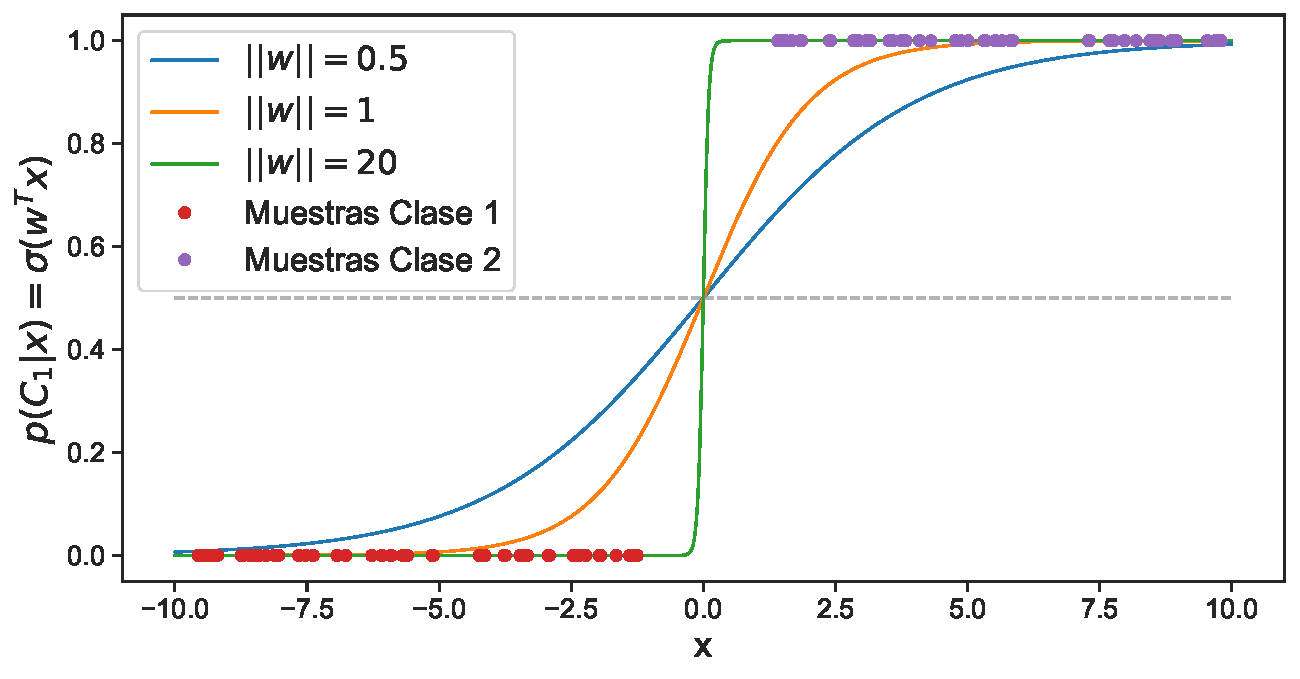
\includegraphics[width=0.9\textwidth]{../img/cap3_logistica.pdf}\\
  \caption{En gris la frontera de decisión: una nueva entrada $x_\star$ será asignada a la clase $\cC_1$ si $p(\cC_1|x_\star)>\frac{1}{2}$, en caso contrario, será asignada a $\cC_2$. Se observa que al entrenar con más muestras, $\norm{w}$ crece por lo que el parámetro se sobreajusta a los datos y el clasificador converge a una función indicatriz.}
\end{figure}


\end{frame}

\begin{frame}
  \titlepage
\end{frame}



%Quitar de comentarios apenas se agregue alguna referencia 
%\bibliography{../capitulos/referencias} %Bibliografía
%\bibliographystyle{apacite}
\end{document} 